\section{Intro to IoT}

\begin{frame}{Introduction to IoT}
	\begin{itemize}
		\item IoT is a connecting \textbf{things} to internet
		\begin{itemize}
			\item Example: Mobile phone
			\item It was initially used only for two-way vice communication
			\item Now it connects to internet too!
			\item Its a \textbf{thing}, which is connected to \textbf{internet} $\Rightarrow$ IoT
		\end{itemize}
		\item Two types:
		\begin{itemize}
			\item Device computes locally and interacts on internet
			\item Device does not compute locally but interacts on internet
		\end{itemize}
		\item Interaction on internet means:
		\begin{itemize}
			\item Write and read data
			\item Write and read code to control systems
		\end{itemize}
	\end{itemize}
\end{frame}

\begin{frame}
	\begin{itemize}
		\item Open Source hardwares
		\item Two examples:
		\begin{itemize}
			\item Arduino
			\item RPi
		\end{itemize}
		\item We shall use RPi in this workshop
		\begin{itemize}
			\item It has lot more features!
		\end{itemize}
		\item Lets see how RPi is different than Arduino
	\end{itemize}
\end{frame}

\begin{frame}{Arduino vs RPi}
	\begin{table}
		\centering
		\begin{tabular}{|l|l|l|}
			\hline
			\textit{Feature} & \textbf{Ardunio} & \textbf{RPi} \\ \hline
			\textbf{Processor} & 16MHz & 900 MHz \\ \hline
			\textbf{Resolution} & 8 bit & 32 bit \\ \hline
			\textbf{Memory} & 32 K Flash, 2K SRAM & 4GB flash, 512K SRAM \\ \hline
			\textbf{Voltage level} & 5V & 3.3 V \\ \hline
			\textbf{Interface} & No OS & Has OS \\ \hline
		\end{tabular}
	\end{table}
\end{frame}

\begin{frame}{OS}
	\begin{figure}
		\centering
		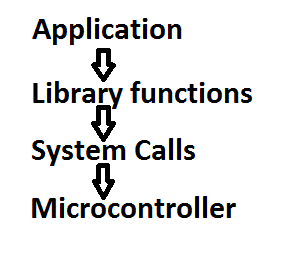
\includegraphics[width=6cm,height=6cm,keepaspectratio]{os}
		\caption{Working of OS}
	\end{figure}
\end{frame}

\begin{frame}{Arduino vs RPi}
	\begin{itemize}
		\item Arduino has only an Application and a Micro-controller
		\begin{itemize}
			\item Application directly controls the pins
		\end{itemize}
		\item RPi has two extra layers i.e library functions and systems calls
		\begin{itemize}
			\item Application does not directly control the pins
			\item Application needs to call a library function, which in turn calls systems calls to control pins
			\item \textbf{Not real time}
			\item \textit{Consumes a lot of memory for OS}
		\end{itemize} 
	\end{itemize}
\end{frame}

\begin{frame}{Advantages of having OS on board}
	\textcolor{blue}{User Interface}
	\begin{itemize}
		\item Can use small programs provided by OS without writing code
		\begin{itemize}
			\item Text based
			\begin{itemize}
				\item Write commands to perform tasks
			\end{itemize}
			\item GUI-based
			\begin{itemize}
				\item Point-click actions to perform tasks
			\end{itemize}
		\end{itemize}
		\item \textbf{Why use text based interface if you have GUI}
		\begin{itemize}
			\item GUI provides only a small feature of control over OS
			\item Command line provides full feature control
			\begin{itemize}
				\item But one needs to memorize a \textbf{large} set of commands
			\end{itemize}
		\end{itemize}
	\end{itemize}
\end{frame}

\begin{frame}{Advantages of having OS on board}
	\textcolor{blue}{Multiple processes}
	\begin{itemize}
		\item Can execute many processes concurrently
		\begin{itemize}
			\item In Arduino, only one programs runs at a time
			\item One needs to put all the features in a single program
			\item In RPi, one can make a lot of small programs and call them from a master program at will
			\item When one has a single core, multi-processing does not mean all processes running \textbf{at same time}
			\item Time given to all processes is swapped so fast that we don't feel the difference
			\item Advantage
			\begin{itemize}
				\item Can run some processes in background while doing important tasks
			\end{itemize}
		\end{itemize}
	\end{itemize}
\end{frame}

\begin{frame}{Advantages of having OS on board}
	\textcolor{blue}{Easier changing hardware connected}
	\begin{itemize}
	\item User Application $\Rightarrow$ /dev/\textcolor{blue}{xxx} $\Rightarrow$ Device driver $\Rightarrow$ Hardware device
	\item \textcolor{blue}{xxx} is a file associated with a hardware device
	\item User simply interacts with all devices by accessing the file
	\item Every device is accessed in a uniform way
	\begin{itemize}
		\item User simply interacts with file for device
		\item File contains code to interact with device driver
		\item The burden to working with device rests with the file
	\end{itemize}
	\item Device driver is the code for accessing physical features of devices
\end{itemize}
\end{frame}

\begin{frame}{Intro to RPi}
	\begin{itemize}
		\item Microcomputer
		\begin{itemize}
			\item Credit card sized ($20 \times 10$ cm)
			\item Weight = $68$ g
		\end{itemize}
		\item Very cost effective
		\begin{itemize}
			\item Presently available for INR $2,875$ at amazon 
		\end{itemize}
		\item Low power consumption 
		\begin{itemize}
			\item We will use mobile phone charger
		\end{itemize}
		\item Remote access over internet
		\begin{itemize}
			\item We will use a LAN cable for connectivity
		\end{itemize}
		\item Runs Linux
		\begin{itemize}
			\item Raspbian is a version of Debian optimized for RPi
		\end{itemize}
	\end{itemize}
\end{frame}

\begin{frame}{Versions of RPi boards}
	\begin{table}
		\centering
		\begin{tabular}{|l|l|}
			\hline
			\textbf{Name} & \textbf{Release date} \\ \hline
			\textcolor{red}{RPi 1 Model A} & February 2012 \\ \hline
			RPi 1 Model A+ & November 2014 \\ \hline
			\textcolor{red}{RPi 1 Model B} & April-June 2012 \\ \hline
			RPi 1 Model B+ & July 2014 \\ \hline
			\textcolor{blue}{RPi 2 Model B} & February 2015 \\ \hline
			RPi zero & November 2015 \\ \hline
		\end{tabular}
	\end{table}
\end{frame}

\begin{frame}{Powerful IoT platform}
	\begin{itemize}
		\item Broadcom $900$ MHz BCM$2836$ ARMv$7$ Quad Core Processor SoC 
		\item Broadcom VideoCore IV GPU
		\item $1$ GB RAM
		\item Expanded $40$-pin GPIO Header
		\item $4$ x USB$2.0$ Ports with up to $1.2$A output
		\item $4$ pole Stereo output and Composite video port
		\item Full size HDMI
		\item CSI camera port for connecting the Raspberry Pi camera
		\item DSI display port for connecting the Raspberry Pi touch screen display
		\item Micro SD port for loading your operating system and storing data
		\item Micro USB power source
	\end{itemize}
	Ref: \url{https://www.raspberrypi.org/products/raspberry-pi-2-model-b/}
\end{frame}

\begin{frame}{RPi}
	\begin{figure}
		\centering
		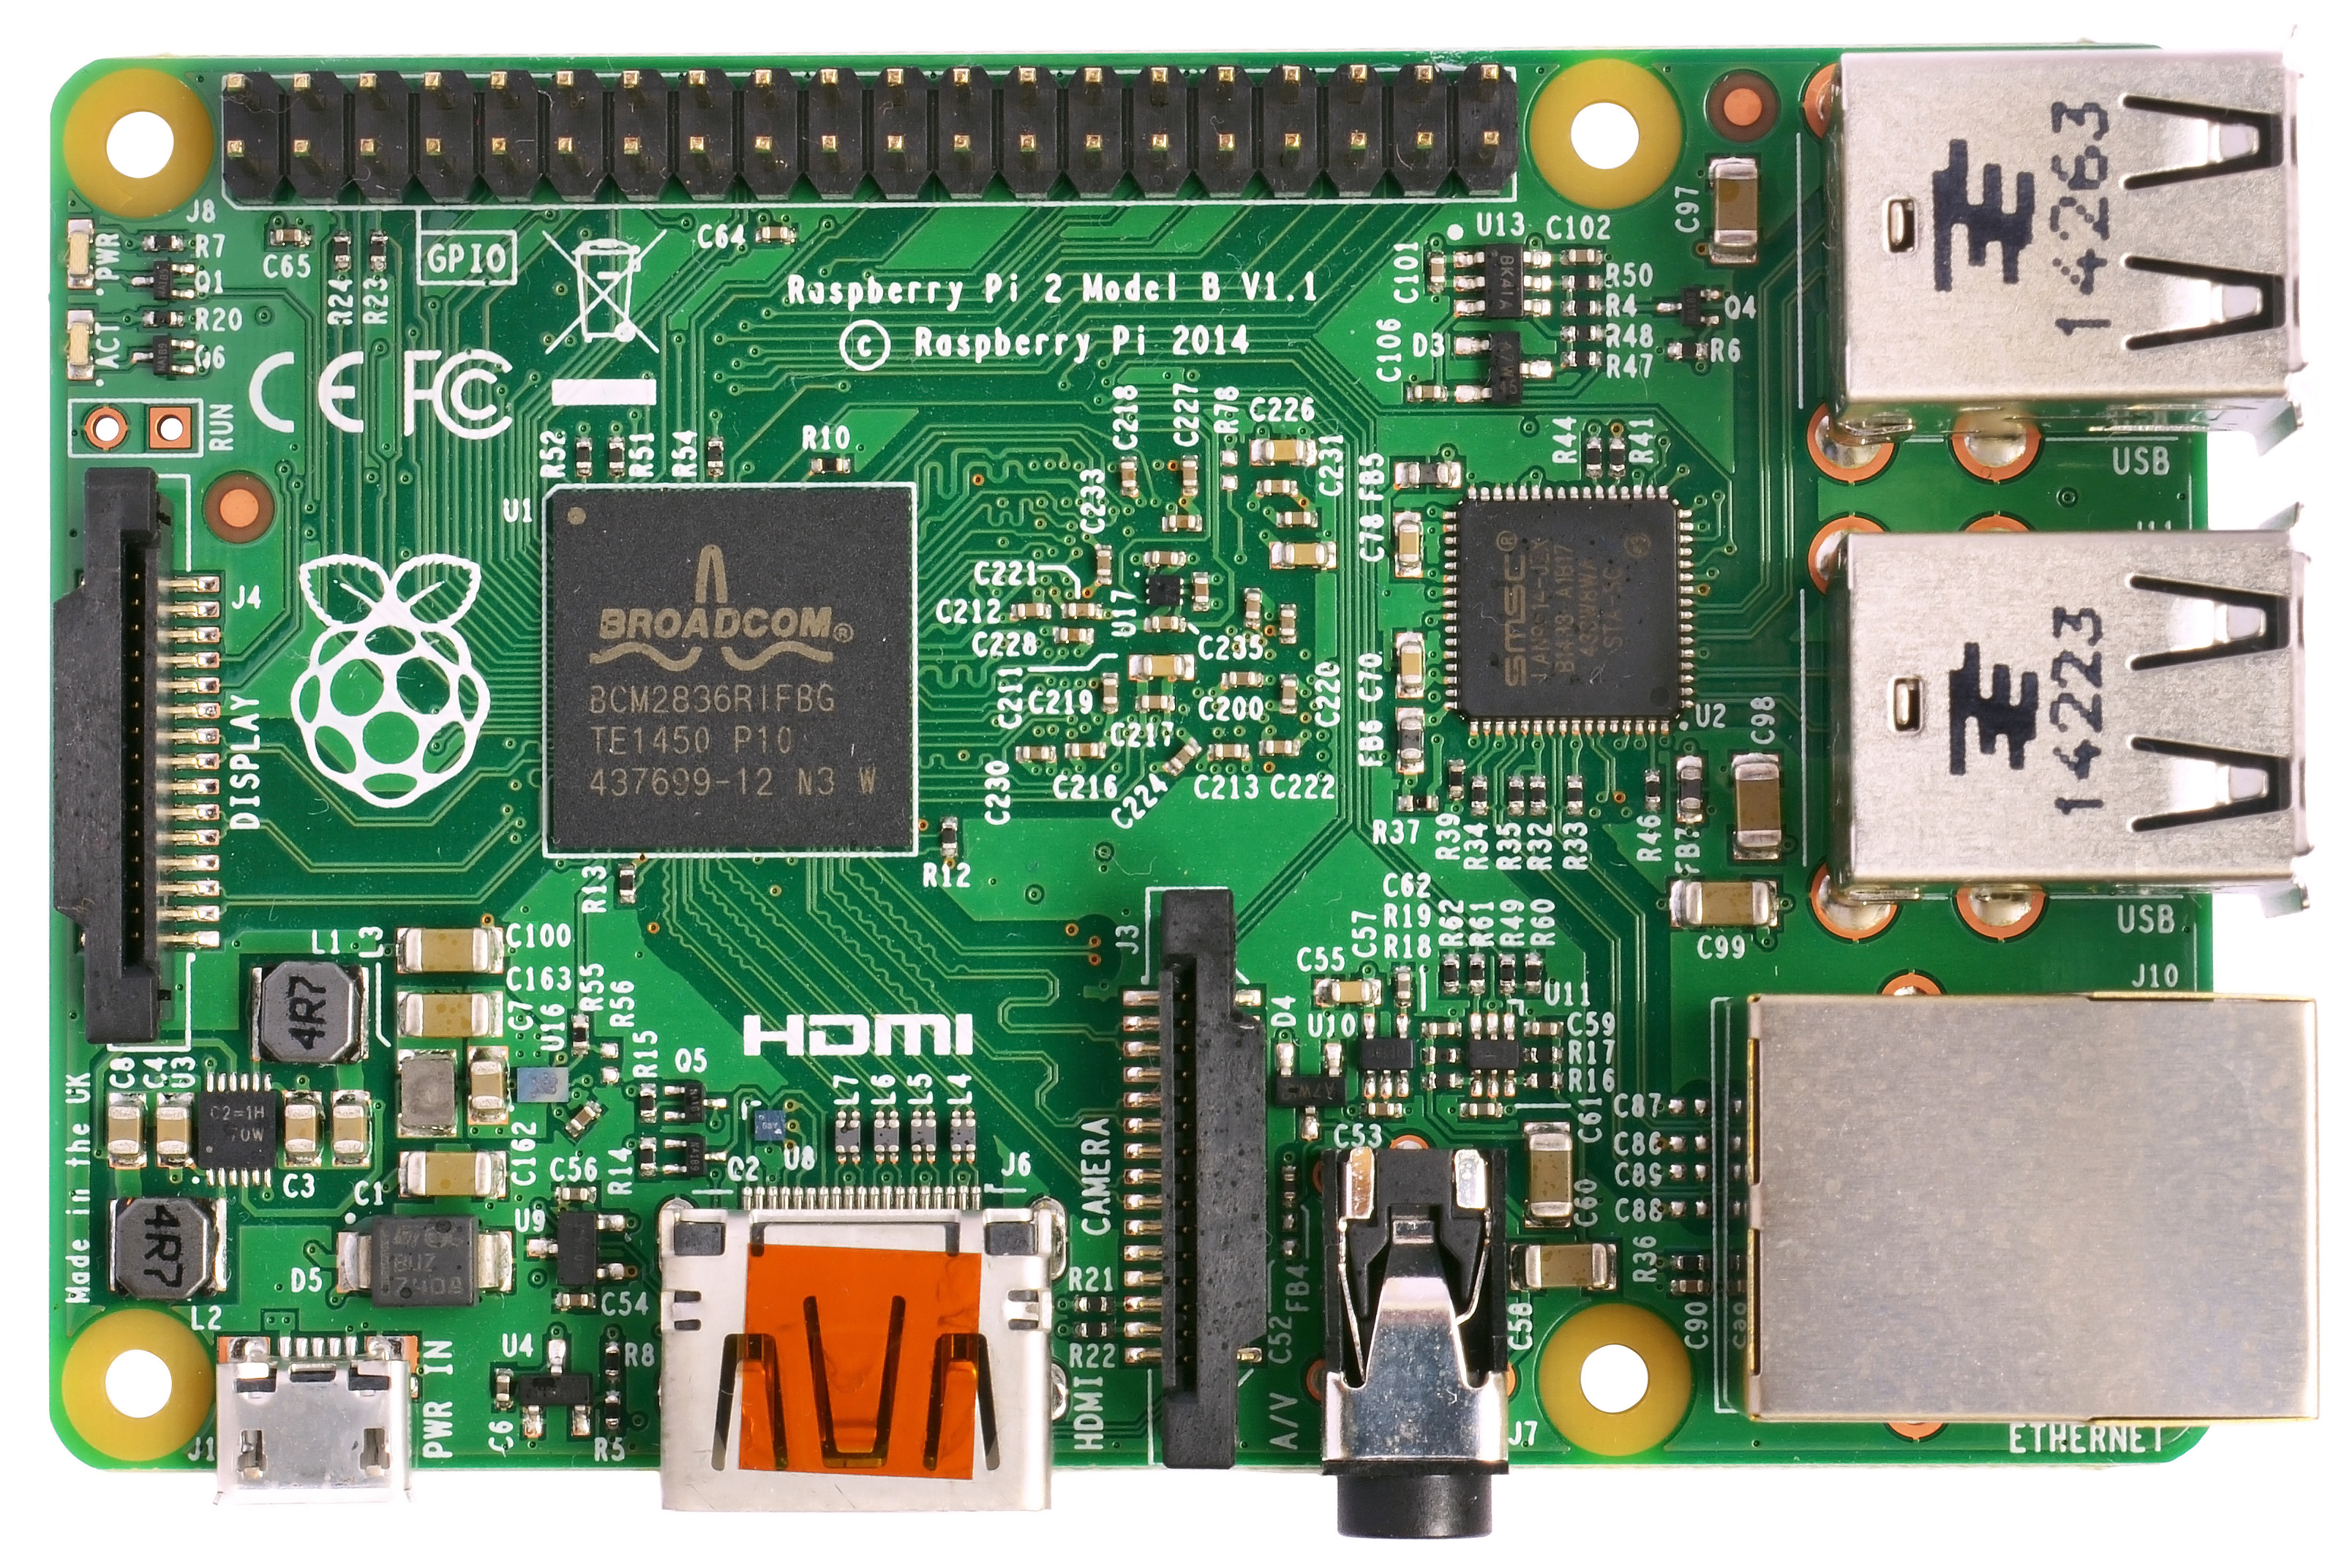
\includegraphics[width=10cm,height=10cm,keepaspectratio]{RPi2}
		\caption{Top portion of Raspberry Pi 2 Model B}
	\end{figure}
\end{frame}

\begin{frame}{OS}
	\begin{itemize}
		\item OS is installed on a micro SD card
		\item Raspbian is optimized OS for RPi
		\item Available at \url{https://www.raspbian.org/}
		\item Micro SD cards with pre-installed OS are also available
		\item Installation
		\begin{itemize}
			\item Format the card
			\item Install NOOBS
			\item Choose Raspbian
			\item Install
		\end{itemize} 
	\end{itemize}
\end{frame}

\begin{frame}{Hardware Connections}
	\begin{itemize}
		\item Monitor
		\begin{itemize}
			\item Using HDMI cable, connect a monitor/projector
			\item If monitor has VGA port, use a VGA-HDMI adapter
		\end{itemize}
		\item Keyboard and mouse
		\begin{itemize}
			\item If you have wired keyboard and mouse, connect them individually to two USB ports
			\item If you have set of wireless keyboard and mouse, use one USB port for adapter
		\end{itemize}
		\item SD card
		\begin{itemize}
			\item Use SD card slot on back side
			\item Use 4GB + card for better performance and enough storage
		\end{itemize}
		\item Power
		\begin{itemize}
			\item Use a 5 V 2 A charger
		\end{itemize}
	\end{itemize}
\end{frame}

\begin{frame}{Setup}
	\begin{enumerate}
		\item Plug in monitor(HDMI), keyboard (USB), mouse (USB)
		\item Get OS on a formatted microSD card
		\begin{itemize}
			\item Format micro SD card using a SD reader
			\item Use NOOBS (New Out-Of-Box Software)
			\item Download from \url{https://www.raspbian.org/downloads}
			\item Extract NOOBS download
			\item Put it in micro SD card
		\end{itemize}
		\item Plug Micro SD card in RPi
		\item Power ON the RPi
		\item NOOBS GUI starts running on screen
		\item NOOBS will install an OS on your micro SD card
		\begin{itemize}
			\item Will offer a list of options
			\item If you are connected to internet, it will offer a longer list
			\item Click \textbf{Raspbian} and install
		\end{itemize}
	\end{enumerate}
\end{frame}

\begin{frame}{Configuring RPi}
	\begin{itemize}
		\item First time RPi boots up, it runs a tool called \textbf{raspi-config}
		\begin{itemize}
			\item Used to configure RPi
			\item Defines username, password etc.
			\item Can be invoked at any stage by writing raspi-config on terminal
			\item Expand file system
			\begin{itemize}
				\item Reformats micro SD card file system to access all the memory
			\end{itemize}
			\item Change User account
			\begin{itemize}
				\item Default username is \textbf{pi} and password is \textbf{raspberry}
			\end{itemize}
			\item Enable boot to Console/Destop/Scratch
			\begin{itemize}
				\item Console is default boot option
				\item Choose Desktop
				\item Scrach is a programming langauge for kids
			\end{itemize}
			\item Internationalization and Rastrack
			\begin{itemize}
				\item Change Locale
				Change timezone
				Change keyboard Layout
			\end{itemize}
			\item Add to Rastrack
			\begin{itemize}
				\item Service which allows RPi users to find one another based on IP location
				\item Optional
			\end{itemize}
		\end{itemize}
	\end{itemize}
\end{frame}

\begin{frame}{Over Clocking}
	\begin{itemize}
		\item Increasing clock frequency of device beyond recommendation
		\item There are a lot of clocks in RPi
		\item Example:
		\begin{itemize}
			\item ARM frequency
			\item SDRAM frequency
		\end{itemize}
		\item Impact
		\begin{itemize}
			\item Instructions are executed faster
			\item About one instruction is executed per clock time period
		\end{itemize}
		\item Risk
		\begin{itemize}
			\item Signals might not reach destination on time
			\begin{itemize}
				\item Whole machine fails
			\end{itemize}
			\item Heating
			\begin{itemize}
				\item Lifetime of device gets shortens
			\end{itemize}
		\end{itemize}
	\end{itemize}
\end{frame}